\subsection{Instruction Solver}

%\jled{How sample programs used in here? No mention.}
We wrote a simple PTX code generator, which generates PTX code with various modifiers specified.
Then compile PTX file to cubin by {\tt ptxas}, and disassemble it by {\tt cuobjdump} to generate real assembly. 
As Figure~\ref{fig:imm} shows an assembly instruction consists of three fields: {\tt opcode}, {\tt operand} and {\tt modifier}. We express these information in a struct
varaible $instMap$, which is input of our solver.
%In this way, we generate real assembly instruction and their 64-bit encoding, which is the input of solver algorithm.
%We disassmble libcublas.so to generate instruction and their corresponing 64-bit encodings. There are $1537123$ different encodings of cublas 7.0 library in total.

An operand could be register({\tt R5}), 
global memory({\tt [R6+0x20]}), constant memory({\tt C[0x2][0x40]}), shared memory ({\tt [0x50]}),
immediate values({\tt 0x9} and{\tt1.5}), or predicate register({\tt P3})~\cite{ptx2015isa}. %represented by different .
And we observe the name of operand is always related with a number, hence the encoding of operand can be inferred by its name.
For instance, the register operand {\tt R5} is inferred as $101$ in binary format, while immediate value {\tt 0x9} is $1001$. 
%Besides, the fixed lengths of these fields allow us to determine their positions \jled{and lengths, don't need to specify lengths here.} relatively easily and hence to encode them. 
The encodings of opcodes and modifiers are mnemonic symbols, therefore, they can not be speculated by names. 
They must be enumerate in their encoding space, and we design a heuristic algorithm on a pruned search space to
determine the position of opcode and modifier.
Modifiers are instruction-sensitive, that is modifiers in the same type may be different encodings for different instructions. 
For instance, masks of type-size
modifier for {\tt LD} and {\tt LDG} are at different binary positions. Hence, we process each instruction's modifier separately. 

\begin{algorithm}[htbp]
    \caption{Immediate Solver} %\jled{what about changing ``pushback'' to ``put'' with an increment for p?} \jled{What about use register solver for this algorithm?}}
      \label{algo:int_solver}
  \begin{algorithmic}[1]
      % \LineComment {input is pairs of full instruction and 64-bit encoding}
      % \LineComment {output is the position of immediate}
	  \State \textbf{Input:} instMap (A map of immediate instructions and their 64-bit encodings)
      \State \textbf{Output:} immediate operand's binary position
      \State $cPos$ $\gets$ \{\} \Comment{record current positions}
      \State $pPos$ $\gets$ \{0,1,2,...63\} \Comment{all potential positions}
	  % \LineComment {check if position is unique}
      \While {length($pPos$) $>$ 1}
      % \While {$pPos$ $\neq$ NULL}
      \LineComment {fetch a random immediate instruction}
      \State $inst$ $\gets$ $instMap[random()]$ 
      \State $enc$ $\gets$ $inst.enc64$ \Comment{64-bit binary encoding}
      \State $imm$ $\gets$ $inst.imm$ \Comment{immediate value}
	  \LineComment {express immediate in its complement code}
      \State $immB$ $\gets$ complement($imm$)
      \State $p$ $\gets$ 0
      % \State $immLen$ $\gets$ length($immBin$)
      % \LineComment {match immBin in 64-bit encoding}
      \LineComment {find all the matching positions}
      \While {$p+$ length($immB$) < $64$}
      \If {strcmp($immB,enc+p$)}
      \State put(p, cPos); $p$ $\gets$ $p+1$;
      \EndIf
      \EndWhile
      \LineComment {common positions of cPos and pPos}
      \State $cPos$ $\gets$ $cPos$ $\cap$ $pPos$
      \State $pPos$ $\gets$ $cPos$
      \State $cPos$ $\gets$ \{\}
      \EndWhile
      \State \textbf{Return} $pPos[0]$
  \end{algorithmic}
\end{algorithm}
\subsubsection{Operand: Fixed Length Field}
Algorithm~\ref{algo:int_solver} shows pseudocode for immediate typed operand decoding process. 
The basic idea is that match binary encoding of operand in $64$ instruction encoding and find
position until the postion is unique. The input instructions are from disassembly code (i.e., NVIDIA CUBLAS library).
First, we randomly pick up an instruction that has the field we want to probe, and represent the field in binary by its 
name. Second, we match the operand binary in $64$-bit instruction encoding, and find possible positions. Third, we 
intersect current candidates with previous ones, if the number of candidates is $1$, we find the position. Otherwise, 
we set the current candidate to the previous one and randomly pick next instruction to repeat the procedure.
Other operand type such as register operand can be use similar routine by matching the corresponding operand binary.

Once operand position is found, we need to probe or verify the length of operand encoding. Some are easy to be
deduced, for example, each thread can use at most $256=2^{8}$ registers, we could predict the length of register 
operand mask to be $8$.
However, other operand types like immediate $0x48$ or subscript of constant memory $C[0x2][0x05]$, are more complicated 
to predicate. Our solution is to set the bit from the position bit by bit to check whether the operand value is grown 
as we expected. For instance, by using Algorithm~\ref{algo:int_solver}, we find out that the immediate operand position 
of {\tt IADD RX, RY, 0ximm} (the RX and RY are arbitrary register operands, 0ximm is immediate operand) is at bit $23$ 
as shown in Figure~\ref{fig:imm}. As specified in~\cite{cuda2015programming}, NVIDIA GPU uses little-endian 
representation, then we set the bits higher than the $23$ to $1$ bit by bit, and observe the the disassembled code. 
Immediate value increases continuely until reaches value {\tt 0x7ffff}, which means that $41\sim23$ is for integer 
immediate.%No {\tt fffff} immediate was got even if we set bit $42$ to be $1$.  

\begin{figure}[htbp]
\begin{center}
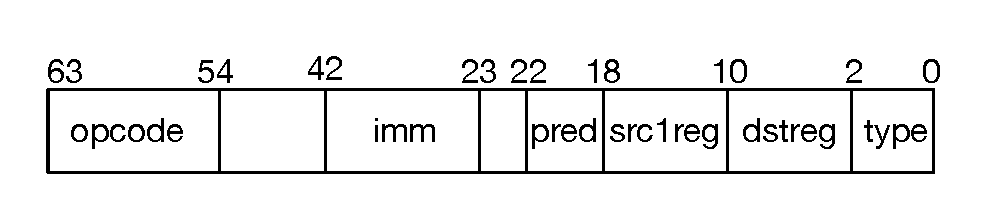
\includegraphics[scale=0.5]{imm}
    \caption{Immediate position at {\tt IADD} instruction}
\label{fig:imm}
\end{center}
\end{figure}

\subsubsection{Opcode}
Unlike operand, opcodes and modifiers do not show their encodings literally. One possible way to crack the operand 
encoding is to write intermediate codes
based on NVIDIA PTX syntax, and generate encoding by using NVDIA toolchain.
Then, opcode can be got by stripping out operand mask, and flag can be found by stripping out both opcode and operand 
mask. However, the uncompleteness of NVIDIA document hinders us to find out all the opcodes and instruction modifiers. 
Another feasible way is to emulate all of possible binary combinations after striping out operand mask.
In general, each instruction has $3$ register operands, and one 4-bit predicate register, $64-8*3-4=36$ bits are left 
to probe.
In fact, we can further prune the search space by recognizing possible position by algorithm~\ref{algo:opcode}. By 
randomly probing bit by bit, we find that both the top $10$ bits and lower $2$ bits represent opcode.
%and other bits represent flags. 
Thus, we only enumerate these opcode bits which generate a acceptable search space. Finally, we find 
the minimal opcode without any flags. 

\begin{algorithm}[htbp]
      \caption{Opcode Solver}\label{algo:opcode}
  \begin{algorithmic}[1]
      \State \textbf {Input:} instMap (A map of instructions and their 64-bit encodings)
      \State \textbf {Onput:} Opcodes' positions in 64-bit encoding
      \For {$i \gets 0, N$}
	  %\LineComment {fetch an instruction from generated database \jled{what's the database?}}
      \State $inst \gets instMap[i]$
      \State $enc \gets inst.enc64$
	  \LineComment {check each bit of $enc$ for opcode}
      \For {$j \gets 0, 63$}
      \LineComment {if bit $j$ not operand bit and its value is 0} % \jled{what about enc[j]!=0? No need to check if it is opcode?}}
      \If {notOprd($enc[j]$) and $enc[j] = 0$}
      \LineComment {set bit $j$ to $1$}
      \State nEnc = setbit($enc, j, 1$)
	  \LineComment {disassemble new encoding nEnc}
      \State nInst=nvdisasm(nEnc)
	  \LineComment {bit $j$ belongs to an opcode if it is changed }
      \If {$nInst.op\neq inst.op$}
      \State put($j$, $opBits$)
      \EndIf
      \EndIf
      \EndFor
      \EndFor
      \State \textbf{Return} opBits %\jled{All instructions' opcodes are stored in opBits?}
  \end{algorithmic}
\end{algorithm}

\subsubsection{Modifier: Instruction Specific}

Modifier(also called flags) defines a specific behavior for an instruction. For example,
{\tt LD} instruction has type-size modifiers, such as {\tt .u8}, {\tt .s8}, {\tt .u16}, {\tt .32}, {\tt .64} and {\tt 
.128}. {\tt LD} also has cache operation modifier, such as {\tt .CS}(cache streaming) and {\tt .cg}(cache at global 
level). Modifiers are much more complicated because its position spans accross the reminding bits and one instruction 
may have more than one kinds of modifiers. By excluding both opcode and operand mask, there remain around $24$ bits. In 
order to reduce search space, we observe that the default value for modifier is $0$. That is, modifier works when at 
least one bit is set. We can check possible positions of modifiers by greedily set the remaining bits one by one to 
observe whether flags will change.
